\documentclass{standalone}
\usepackage{tikz}

\begin{document}

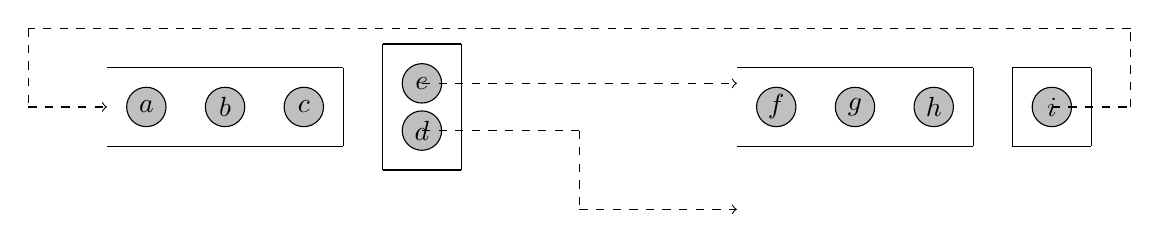
\begin{tikzpicture}
  \draw (0, 0) -- (3, 0);
  \draw (3, 0) -- (3, 1);
  \draw (0, 1) -- (3, 1);
  \filldraw [fill=black!25, draw=black] (0.5, 0.5) circle [radius=0.25] node {$a$};
  \filldraw [fill=black!25, draw=black] (1.5, 0.5) circle [radius=0.25] node {$b$};
  \filldraw [fill=black!25, draw=black] (2.5, 0.5) circle [radius=0.25] node {$c$};
  \draw (3.5, -0.3) -- (3.5, 1.3);
  \draw (3.5, 1.3) -- (4.5, 1.3);
  \draw (4.5, 1.3) -- (4.5, -0.3);
  \draw (4.5, -0.3) -- (3.5, -0.3);
  \filldraw [fill=black!25, draw=black] (4, 0.2) circle [radius=0.25] node {$d$};
  \filldraw [fill=black!25, draw=black] (4, 0.8) circle [radius=0.25] node {$e$};

  \draw (8, 0) -- (11, 0);
  \draw (11, 0) -- (11, 1);
  \draw (8, 1) -- (11, 1);
  \filldraw [fill=black!25, draw=black] (8.5, 0.5) circle [radius=0.25] node {$f$};
  \filldraw [fill=black!25, draw=black] (9.5, 0.5) circle [radius=0.25] node {$g$};
  \filldraw [fill=black!25, draw=black] (10.5, 0.5) circle [radius=0.25] node {$h$};
  \draw (11.5, 0) -- (11.5, 1);
  \draw (11.5, 1) -- (12.5, 1);
  \draw (12.5, 1) -- (12.5, 0);
  \draw (12.5, 0) -- (11.5, 0);
  \filldraw [fill=black!25, draw=black] (12, 0.5) circle [radius=0.25] node {$i$};

  \draw [dashed] (4, 0.2) -- (6, 0.2);
  \draw [dashed] (6, 0.2) -- (6, -0.8);
  \draw [dashed, ->] (6, -0.8) -- (8, -0.8);
  \draw [dashed, ->] (4, 0.8) -- (8, 0.8);
  \draw [dashed] (12, 0.5) -- (13, 0.5);
  \draw [dashed] (13, 0.5) -- (13, 1.5);
  \draw [dashed] (13, 1.5) -- (-1, 1.5);
  \draw [dashed] (-1, 1.5) -- (-1, 0.5);
  \draw [dashed, ->] (-1, 0.5) -- (0, 0.5);
\end{tikzpicture}

\end{document}
